\documentclass[journal]{IEEEtran}

\usepackage{biblatex}

\usepackage[fleqn]{amsmath}
\usepackage{amssymb}
\usepackage{graphicx}
\usepackage{cancel}
\usepackage{tabularx}

\usepackage{caption}
% \usepackage{subcaption}

\usepackage{subfig}
\addbibresource{./citations.bib}

% \graphicspath{ {C:/Users/jonat/Documents/ECH-267-Adv.-Proc.-Control/Project/1_Report/images/}}
\graphicspath{ {C:/Users/Indy-Windows/Documents/ECH-267-Adv.-Proc.-Control/Project/1_Report/images/}}

\usepackage{hyperref}
\hypersetup{
colorlinks=false,
linkcolor=blue,
filecolor=magenta,
    urlcolor=blue,
}
\urlstyle{same}

% \hyphenation{op-tical net-works semi-conduc-tor}


\begin{document}

\title{MPC for Robotic Arm Path Planning and Control \\ ECH-267 Final Project Report}


\author{Jonathan~Dorsey \IEEEmembership{Member: No Sleep Club: est. 2017} \\  \url{https://github.com/JonnyD1117/ECH-267-Adv.-Proc.-Control/tree/main/Project}}


% The paper headers
\markboth{Journal of Graduate School Assignments, March~2021}%
{Dorsey \MakeLowercase{\textit{et al.}}: MPC for Robotic Arm Path Planning and Control ECH-267 Final Project Report}

% make the title area
\maketitle

% As a general rule, do not put math, special symbols or citations
% in the abstract or keywords.
\begin{abstract}
  The objective of this project is to implement a simulated optimal \underline{Path Planner} using Model Predictive Control (MPC) to plan and control the behavior of a 2 degree of freedom (2DOF) robotic arm. The responsibility of the MPC planner will be to generate the `optimal' path and to drive the arm from its current position to the next. The main challenges faced in completing this project consist of solving for the \textbf{nonlinear equations of motion} (as well as any required forward/inverse kinematics) of the robotic arm as well as formulating and solving the \textbf{MPC controller}, at each timestep, both control and planning using the CasADi optimization framework, to test the scenario of simulated real-time performance.
\end{abstract}

% Note that keywords are not normally used for peerreview papers.
\begin{IEEEkeywords}
Model Predictive Control, Robot Arm, Lagrange Equations, Path Planning, Obsticle Avoidance, DH Parameters, Trajectory Generation.
\end{IEEEkeywords}


\IEEEpeerreviewmaketitle

\section{Introduction}

\IEEEPARstart{T}{he} world of robotics is full of constraints, demands, and performance trade-offs that humans handle naturally on a daily basis. Unlike humans, robots require control and planning strategies which are flexibility enough to work around constraints and limitations, while accurately meeting control and performance objectives in uncertain environments. While the emergence of machine learning techniques and methods offers promise of stateoftheart improvements and performance, most robotic systems still demand a more practical and robust planning and control algorithms, capable of offering a compromise between the performance criteria, flexibility to navigate constraints, and amount of computational power required to compute valid control commands in real-time. \\

In the world of robot manipulators, tasks can range from relatively simple and coarse motions to extremely complex and detailed actions. One common control strategy which has seen great success, in robotics, in recent years is Model Predictive Control (MPC). MPC is an optimal control methodology which solves the a given optimal control problem (OCP) in a receding fashion, over a finite horizon. While these controllers are far more sophisticated than standard classical or modern control strategies, the increased complexity and computation can be applied to a wider class of control problems. This flexibility in natively handling constraints as well as naturally extending to nonlinear and multiple-input-multiple-output-systems makes MPC an attractive candidate control methodology for the vast world of robotics where tasks can range from autonomous mobile vehicles to robotic manipulators. While MPC has the obvious conns of requiring an approximate solution to an optimization problem, at each time step, the benefits which this methodology offers often make it a viable solution even with the added computationally expense. \\

While control is an important aspect of modern robotics, it is often more valuable to have an understanding of the intent or future actions which an autonomous system believes it should take, to accomplish a goal. In general, this problem is known as \textbf{path planning}, and is an important part of modern robotics research. Many modern path planning approaches use a vast array of different planning paradigms, such as discretization, graph, probablistic, and heuristic methods which have all shown great promise, and present there own unique benefits and limitations. Often in the more general case of motion planning, it is desirable to not only control the position, but also the velocity and acceleration of a system, in both space and time. However, for the purpose of this paper, only the more restricted case of path planning (e.g. position planning) will be considered.  \\

To this point, another possible method for path planning is the use of MPC, as a optimal path planner. MPC has the potential to provide much of the same functionality as other planning strategies by implementing desireable behavior into a cost function or functional constraints. The ability to leverage and model predictive controller as a path planning with practically no changes to its implementation as a controller also offers an opportunity for systems using MPC to obtain some path planning capabilities for free.   \\

While MPC has been received enormous amounts of research across many fields, including  robotics, many of the applications in robotics focus MPC on mobile robotics such as drones and autonomous vehicles, with significantly less attention focused on the application of MPC as a controller or a planner for robotic manipulators.

\section{Problem Statement}

This paper will investigate the use of MPC as a general control scheme and its utility as a path planner for a simple two link planar robotic manipulator. By the use of simulation, this paper will develop and identify key elements in understanding some of the benefits and limitations of MPC in the context of articulated robotic manipulators.

\subsection{Planar RR Robotic Arm}

The manipulator used in this paper is a two link planar robot arm subject to gravity, fig.\ref{RRrobot}, commonly known as a \textbf{RR} (revolute-revolute) robot. This model commonly does not include any rigid body dynamics and treats the robot as a system of point masses directly coupled with massless rods. While this configuration is very simple, it is conceptually simple, easy to derive its core dynamics, and facilitates a more focused study on the planning and control elements of the paper. \\

\begin{figure}
    \centering
    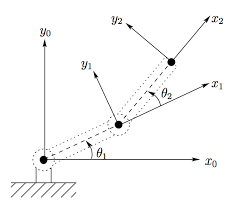
\includegraphics[scale=.5]{2d_arm_2}
    \caption{RR Planar Manipulator subject to gravity}
    \label{RRrobot}
\end{figure}

% \subsection{MPC Control Objectives}
% From a strictly control perspective, this paper seeks to investigate how to formulate MPC for the robot arm, to determine the effectiveness of MPC in , to
%
%
%
% for as a
%
% \begin{enumerate}
%     \item How can MPC be used to control a simple robot?
%     \item How effective is MPC over other control schemes?
%     \item Can MPC be used for obstacle avoidance?
%     \item How long does it take MPC to generate a solution for each time step
% \end{enumerate}
%
% \subsection{Path Planning Objectives}
%
% \begin{enumerate}
%     \item How can MPC be used as a simple path planner
%     \item how reliable is form of path planner
%     \item Can this planner be used reference for
%     \item What restriction on the performance of the sytem does using using this path planner enforce
% \end{enumerate}
%
%
%
%
%
%
% to performance of standard Multiple Shooting MPC on simplified robotic manipulator, quantify the computational burden of implementing MPC, test the flexibility MPC as a framework for advanced control objectives (obstacle avoidance), and to


\section{Background}

To contextualize the implementation of MPC for on robotic manipulators, it is helpful to breakdown a few of the fundamental elements, constructs, and terminology which are commonly used in robotics literature.

\subsection{Robotic Manipulators}

In general robotic arms are classified as either prismatic (linear motion) or revolute (rotational motion) joints. The PUMA 560 [Fig.\ref{puma560}], is an industry standard 6 degree of freedom (DOF) manipulator. It utilizes six revolute joints, connected in a serial fashion. This configuration of only rotating joints makes the PUMA 560 an \textbf{articulated robot}.

\begin{figure}
    \centering
    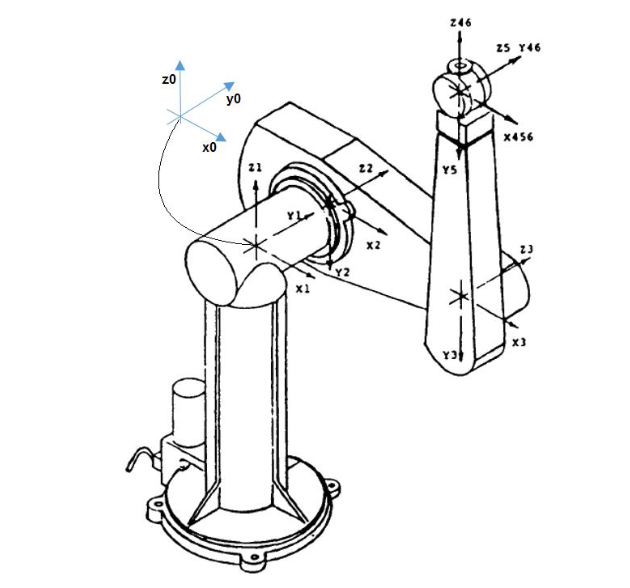
\includegraphics[scale=.5]{puma}
    \caption{Puma560 Robot with Joint Coordinate Frames}
    \label{puma560}
\end{figure}

While the study of high DOF robots is well researched and would be present interesting and complicated scenarios for both control and planning, the scale and complexity of modeling the governing dynamic equations make robots like those in [Fig. \ref{puma560}] impractical for the scope and time restrictions of this paper. This paper, instead, opts to use the dynamically simple RR-robot described above, as its design and test platform for implementing MPC.



\subsubsection{DH Parameters \& Homogenous Transforms}

The Denavit-Hartenberg (DH) parameters are an important tool in describing the geometry of any given robot, and prove to be highly effective in the formulation of joint transformations which enable a concise and universal method for transforming important quanties for kinematic and dynamic analysis of a robot.\\

\noindent The DH Parameters are defined to be...
    $$
    \begin{array}{l}
    a_{i}=\text { the distance from } \hat{Z}_{i} \text { to } \hat{Z}_{i+1} \text { measured along } \hat{X}_{i} \\
    \alpha_{i}=\text { the angle from } \hat{Z}_{i} \text { to } \hat{Z}_{i+1} \text { measured about } \hat{X}_{i} \\
    d_{i}=\text { the distance from } \hat{X}_{i-1} \text { to } \hat{X}_{i} \text { measured along } \hat{Z}_{i} ; \text { and } \\
    \theta_{i}=\text { the angle from } \hat{X}_{i-1} \text { to } \hat{X}_{i} \text { measured about } \hat{Z}_{i}
    \end{array}
    $$


By utilizing the \textbf{homogeneous transform}, which describes the frame position and rotation required to define a vector from one frame to another, we generate a mapping of a vector to or from any coordinate system in the system.

\begin{equation}
    $$
    \left[\begin{array}{c}
    {}^{A}P \\
    1
    \end{array}\right]=\left[\begin{array}{ccc|c}
    {} & {}^{A}_{B}R & & {}^{A}P_{B org} \\
    \hline 0 & 0 & 0 & 1
    \end{array}\right]\left[\begin{array}{c}
    {}^{B}P \\
    1
    \end{array}\right]
    $$
\end{equation}


\begin{equation}
        P = { }_{B}^{A} T^{B} P
\end{equation}

DH parameters can be used to define a single transformation from frame $\{ i\}$ to frame $\{ i-1 \}$, by chaining explicit translations and rotations about specified axes. The matrices $R$ and $D$ represent the homogeneous transformation for rotation and translations repsectively, with the subscript of each providing the axis upon which the operation should be performed.

$$
{ }_{i}^{i-1} T=R_{X}\left(\alpha_{i-1}\right) D_{X}\left(a_{i-1}\right) R_{Z}\left(\theta_{i}\right) D_{Z}\left(d_{i}\right)
$$

This is a powerful concept which facilitates the analysis of any robot whose joints are based on revolute or prismatic members. \\

\subsubsection{Forward \& Inverse Kinematics}

Forward Kinematics (FK) is the study determining the final pose of a manipulator given the individual joint positions and velocities (whether revolute or prismatic). By using DH parameter based transformations, the position or velocity of any joint can computed against the given frame of refernce (often the {0} frame). Forward kinematics is important since it provides a mapping from \textbf{joint space} to the \textbf{task space} of the robot. \\

Inverse Kinematics (IK) is the study of the joint positions given the position and velocity of the manipulator. IK is typically a harder task to perform than FK since there are often multiple solutions which satisfy the pose of the end effector. \\

Both forward an inverse kinematics are important for simulating joint positions and motion of a robot and determining which goal positions are feasible, respectively.

\subsection{Path Planning vs Trajectory Generation}

While frequently used as synonyms, \textbf{path planning} and \textbf{trajectory generation} (in the strict sense) describe two very quantities. A path is typically defined as a sequence of function of position from some point A to another point B. Paths are independent of time and therefore, cannot encode information such as velocity or acceleration, that depend on time. Trajectories, on the other hand, are paths with a dependency on time. Trajectory generation has substantially larger scope than path planning, and possesses substantial body of research.  \\

While trajectory generation is typically of greater utility, as it provides more information about the behavior of system, for the context and scope of this paper, path planning will be a sufficient to describe the behavior of the system from a starting pose to an ending pose.

\section{Methodology}

The methodology followed in this paper consists of deriving the governing equations for the robot, formulating the optimal control problem for MPC, designing the appropriate cost function for the desired behavior, translating this information into CasADi syntax, and numerically simulating the behavior of the robot under MPC control and using the outputs of the MPC to generate paths. Each of these elements is broken down in the following sections.

\subsection{Formulation of Robot Dynamics}
For puposes of this paper, the robot model only includes physical dynamics of the system and not the dynamics of the actuators. It would be relatively simple to derive the actuator dynamics for a more realistic model of how the system operates, but for the purposes of time and simplicity, it is assumed that the joint motors have perfect torque control. \\

As previously mentioned, the model of the robot excludes rigid body effects and only considers the effect of point masses rigidly connected with massless links. Under these assumptions, we can ignore contributions by moments of inertia. This simplifies the process of deriving equations of motion. \\

The Euler-Lagrange Equations are used to derive the explicit dynamics of the system. This variational approach is often more useful and scalable to large and coupled system than classical force and moment balances, since it this method only requires computing the kinetic and potential energies of the system and computing derivatives with respect to generalized coordinates. While equivalent to the Newton-Euler Equations, Lagrange Equations do not require the computing of accelerations. The general form of Lagrange Equations are.
\begin{equation}
\frac{d}{d t} \frac{\partial L}{\partial \dot{\boldsymbol{q}_{i}}}-\frac{\partial L}{\partial \boldsymbol{q}_{i}}=\left[\begin{array}{l}
\tau_{i}
\end{array}\right]
 \quad \quad \text{for i} = 1,2,...
\end{equation}

\noindent Where the lagrangian is the difference between the total kinetic and total potential energy of the system.
\begin{equation}
  L = k - u
\end{equation}

\noindent and where $k$ and $u$ are defined be to...
\begin{equation}
k=\sum_{i=1}^{n} k_{i}
\end{equation}

\begin{equation}
u=\sum_{i=1}^{n} u_{i}
\end{equation}

It should be noted that when defining the individual potential and kinetic terms, they must be written with resepect to the correct frame of reference $\{ i \}$. This can be easily accomplished by using DH parameter homogeneous transformations, previously defined, to write the velocity or position vector of a particular link of the robot with respect to the correct reference frame.
\begin{equation}
k_{i}=\frac{1}{2} m_{i} v_{C_{i}}^{T} v_{C_{i}}+\frac{1}{2}^{i} \omega_{i}^{T} C_{i} I_{i}^{i} \omega_{i}
\end{equation}
\begin{equation}
u_{i}=-m_{i}^{0} g^{T}{ }^{0} P_{C_{i}}+u_{r e f_{i}}
\end{equation}

By computing $i$ Lagrange equations, as expressed above, the equations of motion for the system will be determined. While simple, this process depends on the ability of taking derivatives, which for robotic systems can be highly coupled and result in massive expressions. Typically this would be done using a symbolic math libary or by using the itterative form of the Newton-Euler Equations instead.\\

In general, the serially articulated robots with revolute joints will produce equations of motion (EOM) that take the following form.
\begin{equation}
  \tau = M(\Theta)\ddot{\Theta} + V(\Theta, \dot{\Theta}) + G(\Theta) + F(\dot{\Theta})
\end{equation}


In this formulation, $M$ is the mass matrix which models the effects of mass and moments of inertia which are related to the angular accelerations of the joints. The $V$ vector models the centrifugal and Coriolis forces which are typically functions of velocities, while the $G$ vector models the effects of gravity. Finally, the $F$ vector is added to explictly include the effects of friction/damping, at the joints of each link.

\begin{equation}
\begin{aligned}
M(\theta)=\left[\begin{array}{ll}
 m_{11} & m_{12}  \\
 m_{21} & m_{22} \end{array}\right]
\end{aligned}
\end{equation}

Where

\begin{equation*}
\begin{aligned}
  m_{11} & = m_{1} L_{1}^{2}+m_{2}\left(L_{1}^{2}+2 L_{1} L_{2} \cos \left(\theta_{1}\right)+L_{2}^{2}\right) + \varepsilon \\
  m_{12} & = m_{2}\left(L_{1} L_{2} \cos \left(\theta_{2}\right)+L_{2}^{2}\right) \\
  m_{21} & = m_{2}\left(L_{1} L_{2} \cos \left(\theta_{2}\right)+L_{2}^{2}\right)\\
  m_{22} & = m_{2} L_{2}^{2}+\varepsilon
\end{aligned}
\end{equation*}



\begin{equation}
V(\theta, \dot{\theta})=\left[\begin{array}{c}
-m_{2} L_{1} L_{2} \sin \left(\theta_{2}\right)\left(2 \dot{\theta}_{1} \dot{\theta}_{2}+\dot{\theta}_{2}^{2}\right) \\
m_{2} L_{1} L_{2} \dot{\theta}_{1}^{2} \sin \left(\theta_{2}\right)
\end{array}\right]
\end{equation}


\begin{equation}
G(\theta)=\left[\begin{array}{c}
\left(m_{1}+m_{2}\right) L_{1} g \cos \left(\theta_{1}\right)+m_{2} g_{2} \cos \left(\theta_{1}+\theta_{2}\right) \\
m_{2} g L_{2} \cos \left(\theta_{1}+\theta_{2}\right)
\end{array}\right]
\end{equation}


\begin{equation}
F(\dot{\theta})=\left[\begin{array}{c}
c_{f} \cdot \dot{\theta}_{1} \\
c_{f} \cdot \dot{\theta}_{2}
\end{array}\right]
\end{equation}


It should be noted for simulation purposes, the equations of motion need to express $\tau$ as the input to the robot and the angular accelerations $\ddot{\Theta}$ as the outputs.

\begin{equation} \label{angular_accel}
\ddot{\theta}=(M^{-1})[\tau-V-G-F]
\end{equation}

However, expressing the governing equations in this form result in numerical instabilties during simulation which arise from inverting the mass matrix $M(\Theta)$. Since the mass matrix is a function of angular positions $\Theta$, specific configurations can cause the mass matrix to near a singularity, when inverted. If evaluated numerically, the computed value will explode, typically resulting in the value becoming \textbf{INF} or \textbf{NAN}. To avoid this, the value of $\varepsilon$ can be added to the diagonal terms of $M$ to garuntee that the system will never become singular, during inversion.

By evaluting [eq.\ref{angular_accel}], it is possible to write the nonlinear state space for the robot, as a function of the states $x_{1}=\theta_{1}$, $x_{2}=\theta_{2}$, $x_{3}=\dot{\theta}_{1}$, and $x_{4}=\dot{\theta}_{2}$.

\begin{equation}\label{robot_ss}
\begin{array}{l}
\dot{x}_{1}=x_{3} \\
\dot{x}_{2}=x_{4} \\
\dot{x}_{3}=\ddot{\theta}_{1} \\
\dot{x}_{4}=\ddot{\theta}_{2}
\end{array}
\end{equation}

Where $ \ddot{\theta}_{1}$ and $\ddot{\theta}_{2}$ are defined in APPENDIX???????????.

While still highly nonlinear, [eq. \ref{robot_ss}] encapsulates the complete dynamics of the robot. This formulation can be directly used for numerical simulatation and for use in developing the constraints neccessary for model predictive controller.


\subsection{MPC Formulation}
The mathematical basis for MPC stems from the standard optimal control problem. Under the assumptions that an internal model of the system dynamics exist, that the prediction horizon is finite and proceeds in a receding fashion, the inputs applied to the system, by the controller, are piecewise constant at each time-step, and where the value of the current input is obtained by taking the first value of the optimal input sequence which is obtained by solving the optimization problem at each time-step. This can be written in standard form as...
\begin{equation}
\begin{aligned}
& \min _{n} J_{x}\left(\mathbf{x}_{0}, \mathbf{u}\right)=\sum_{k=0}^{N-1} \ell\left(\mathbf{x}_{\mathbf{v}}(k), \mathbf{u}(k)\right) \\
\text { s.t: }: & \mathbf{x}_{\mathbf{n}}(k+1)=\mathbf{f}\left(\mathbf{x}_{\mathbf{n}}(k), \mathbf{u}(k)\right) \\
& \mathbf{x}_{\mathbf{u}}(0)=\mathbf{x}_{0}, \\
& \mathbf{u}(k) \in U, \forall k \in[0, N-1] \\
& \mathbf{x}_{\mathbf{u}}(k) \in X, \forall k \in[0, N]
\end{aligned}
\end{equation}

In this formulation, the cost function is only propagated to the end of the prediction horizon $N$, from the current initial state of the system. The first equality constraint restricts future states of the system to be feasible with respect to the system model. The second equality constraints requires the initial state of the solver to be the current initial state of the system, while the final constraints require the inputs and states determined by the solver to be valid elements of feasible input and state sets respectively. \\

It should be further noted that this paper uses the \textbf{Multiple Shooting} implementation of MPC as this approach has shown to produce better results and obtained solutions far faster than the naive single shooting approach. This means that the optimization problem has been lifted into a higher dimensional space by including the each state and input over the prediction horizion as a decision variable for the solver. \\

\subsubsection{Cost Function Design}

The general stage cost, as each time-step of the prediciton horizon utilized in this paper follows the typical quadratic form.

\begin{equation}
  \ell\left(\mathbf{x}_{\mathbf{v}}(k), \mathbf{u}(k)\right) = (x-x_d)Q(x-x_d) + (u-u_d)R(u-u_d)
\end{equation}

This parameterization of the stage cost can be further simplified using norm notation.
\begin{equation}
  \ell\left(\mathbf{x}_{\mathbf{v}}(k), \mathbf{u}(k)\right) = \left\Vert x - x_d \right\Vert^{2}_{Q} + \left\Vert u -u_d \right\Vert^{2}_{R}
\end{equation}

The quadratic nature of this cost function is eligant in how simple and intuitive it is comprehend as as well how simple it is to tune using the matrices $Q$ and $R$. \\

However for the scenario testing \textbf{obstacle avoidance}, it is neccessary to append the origin stage cost with an addition term. By adding an obstacle penalty to the stage cost the controller is incentivized to avoid letting the end effector of the robot get too close the specified object. By specifying circular envelopes around the end effector and the obstacle, it is possible to define the minimum distance between the two object such that they do not approach any closer to each other than the sum of radii which define the circular boundaries.

\begin{equation}
\text{min. dist} = -\sqrt{\left(x-x_{0}\right)^{2}+\left(y-y_{o}\right)^{2}}+\left(r+r_{o}\right) \leq 0
\end{equation}

Where $x$ and $y$ constitute the current 2D position of the end effector, while $x_0$ and $y_0$ constitute the \underline{stationary} position of the obstacle. The values of $r$ and $r_0$ define the radii of the circular envelopes enclosing the end effector and obstacle respectively. \\

By using this measure, it is possible to create a penalty such that if the
\begin{equation}
\text{C}(P,P_0) = S(max(\text{min. dist}(P, P_0), 0))^2
\end{equation}

Where $S$ is a large positive weight, and $P$ and $P_0$ are the points defining the end effector and obstacle positions respetively. If the inequality is every violated and the minimum distance between the obstacle and end effector is greater than zero, the magnitude of the distance violation will be used as a penalty in the cost function effectively incentivizing the controller to avoid letting the controller and the obstacle become too close to each other. If the inequality holds, then the value of zero will choosen in the $\text{max()}$ function and will not contribute to the cost function. The final stage cost for obstacle avoidance results in. \\
\begin{equation}
  \ell\left(\mathbf{x}_{\mathbf{v}}(k), \mathbf{u}(k)\right) = \left\Vert x - x_d \right\Vert^{2}_{Q} + \left\Vert u -u_d \right\Vert^{2}_{R} + C(P,P_0)
\end{equation}

While crude, this formulation enables the rudimentary form of obstacle avoidance, if the position of the obstacle is known by the controller. One of the conns of using this penalty in the control law is that the controller is not strictly speaking forbidden (constrained) from violating this minimum distance, but rather is only incentivized by a large penalty to not violate the condition. This is a subtle difference, but time restrictions prevented further exploration of more rigorous constraint formulations such as the use of slack variables. \cite{soft_constraints}

\subsection{Controller Development in CasADi}
In order to solve the optimal control problem, defined above, the CasADi library was utilized to simplify the process of solving optimization problems by use of its symbolic functionality as well as its automatic differentiation, which allow a simple and direct casting of the mathematics into a well structured programming syntax. \\

By leveraging this library and its functionality, it becomes a simple and direct task to cast the MPC formulation into meaning code which can then be feed into a standard optimization solver. For the purposes of this paper, the \textbf{IPOPT} (Interior Point Optimizer) solver was used since it comes prepackaged with CasADi and performs well in a variety of applications.

\subsection{Controller \& Planner Simulation}

Once MPC is implemented via CasADi, numerical simulation merely requires using the first optimal input of the solver, at the initial state, applying that input to a discretized system model, computing the resulting states, updating the current state of the controller, and reapplying the solver for the duration of the simulation time.\\

By virtue of using muliple shooting, the decision variable for this MPC formulation not only includes the inputs over the prediction horizon, but also the corresponding optimal states, according to the model. For the purposes of planning (in simulation) it is possible to directly copy the optimal predicted states directly from the solvers solution, at each time-step, and to use these state sequences as the optimal path, over the duration of the simulation.

\subsection{Controller Testing}

Since the first objective of this paper is to test the efficacy of MPC, there are several interesting scenarios which are of general interest when evaluating how effective MPC based control is, on this type of system. \\

% The controller testing for this section, included nominal performance of MPC as MIMO controller, performance with model/parameter mismatch, the behavior of MPC for infeasible targets, and finally obstacle avoidnace


\begin{enumerate}
    \item Pose-to-Pose Control
    \item Model/Parameter Mismatch
    \item Infeasible Target behavior
    \item Obstacle Avoidance (static)
\end{enumerate}



\subsection{Planner Testing}

The objectives for MPC based path planning are to implement path planning,


\begin{enumerate}
    \item Generate State Prediction Horizon
    \item Create continuous defined path using cubic splines
    \item Test how performance of the system
\end{enumerate}


\section{Results}
\subsection{Controller Results}

\subsubsection{Pose-to-Pose}

As to be expected, the use of MPC on this two link robot, under nominal operating conditions and using a perfect system model performed exceedingly well. As seen in [Fig.\ref{fig:pose2pose}], the controller is able to drive the system from its initial state to the desired final goal to with in an accuracy of .0001\% of the reference value.

\begin{figure}[hb]%
    \centering
    \subfloat[\centering label 1]{{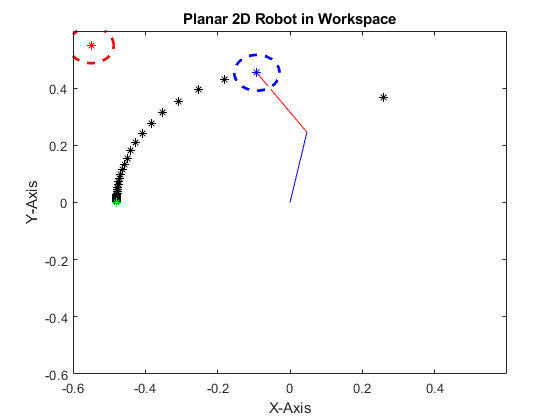
\includegraphics[width=.43\linewidth]{no_obj_path_1} }}%
    \qquad
    \subfloat[\centering label 2]{{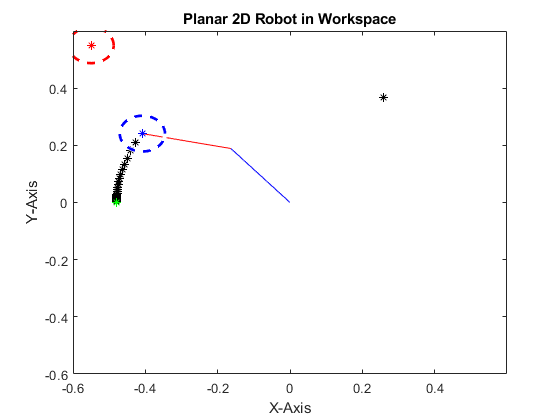
\includegraphics[width=.43\linewidth]{no_obj_path_2} }}%
    % \caption{2 Figures side by side}%
    \\
    \subfloat[\centering label 3]{{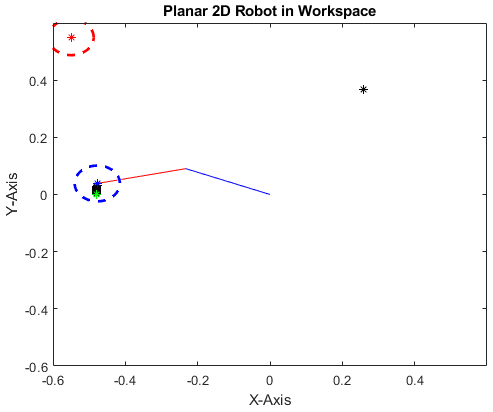
\includegraphics[width=.43\linewidth]{no_obj_path_3} }}%
    \qquad
    \subfloat[\centering label 4]{{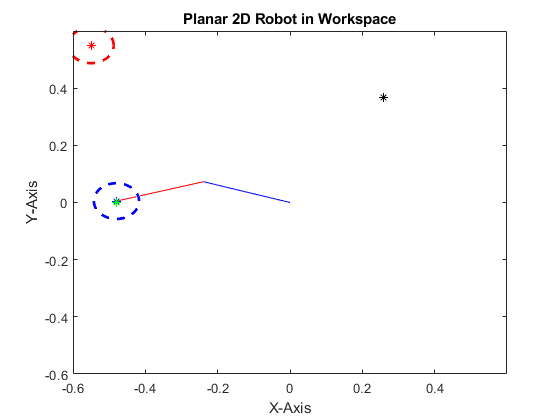
\includegraphics[width=.43\linewidth]{no_obj_path_final} }}%
    \caption{Pose-to-Pose control using MPC}%
    \label{fig:pose2pose}%
\end{figure}

\begin{figure}[ht]%
    \centering
    \subfloat[\centering label 1]{{\includegraphics[width=.43\linewidth]{Nominal_MPC/T1_X_init_25_45_0_0_X_ref_180_n45_0_0/pos} }}%
    \qquad
    \subfloat[\centering label 2]{{\includegraphics[width=.43\linewidth]{Nominal_MPC/T1_X_init_25_45_0_0_X_ref_180_n45_0_0/vel} }}%
    % \caption{2 Figures side by side}%
    \\
    \subfloat[\centering label 3]{{\includegraphics[width=.43\linewidth]{Nominal_MPC/T1_X_init_25_45_0_0_X_ref_180_n45_0_0/tor} }}%
    \caption{Nominal MPC Curves: Ang. Position, Ang. Velocity, Torque}%
    \label{fig:pose2pose_control_action}%
\end{figure}

The plots in [Fig.\ref{fig:pose2pose_control_action}] demonstrate the steady performance of the controller to a constant reference. It should be noted that the torques of the system never converge to zero. This behavior is due to the fact this RR-robot is standing in the vertical plane and is subject to the effect of gravity. This requires the controller to offset the command torques inorder to maintain the commanded position. This would not occur if the robot was oriented in the horizontal plane. In addition, for this reason, certain configurations of initial and goal positions will cause cause the actuator effort to increase or decrease due to the force of gravity working with or against the controller, as a function of the robots initial and goal configurations. \\

\subsubsection{Model/Parameter Mismatch}

One of the other main results, is the steady state performance of the system during model and system parameter mismatch. In this situation the predicted model the controller is using for prediction is not correctly matched to the actual system which the controller is controlling. The results from this study are relatively straightforward. \\

For steady state references, the controller is fairly robust to the parametric uncertainty.

\begin{table}[ht]\caption{Nonlinear Model Results}
    \centering
    \begin{tabular}{c c c c c}
          & Mass1 (kg) & Mass2 (kg) & Link1 (m) & Link2 (m)  \\
        \hline\hline

        Model Params. & .5 & .25 & .25 & .25  \\
        \hline
        & & System Parameters. & & \\
        \hline
        (+5\%)  & .525 & .2625 & .2625 & .2625   \\
        (+10\%) & .55 & .275 & .275 & .275  \\
        (+15\%) & .575 & .2875 & .2875 & .2875 \\
        (+20\%) & .6 & .3 & .3 & .3 \\
        (+25\%) & .625 & .3125 & .3125 & .3125 \\ [1ex]
        (+30\%) & .65 & .325 & .325 & .325 \\ [1ex]

    \end{tabular}
    \label{table:nonlin}
\end{table}


\begin{figure}[ht]%
    \centering
    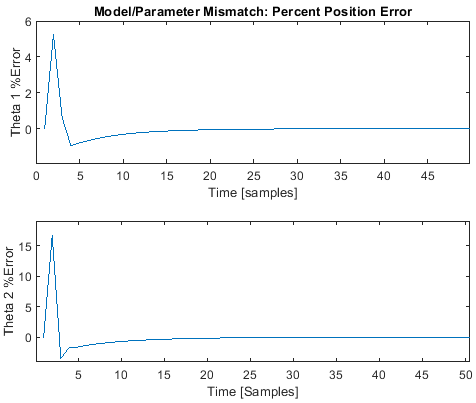
\includegraphics[width=.95\linewidth]{Model Param Mismatch/per_error_pos}
    \caption{Model Parameter Mismatch Steady State Results}%
    \label{fig:model_param_mismatch}%
\end{figure}

\subsubsection{Obstacle Avoidance}

This is obstacle avoidance with MPC

\begin{figure}[ht]%
    \centering
    \subfloat[\centering label 1]{{\includegraphics[width=.43\linewidth]{OBS_Avoid_TEST/T6/pos} }}%
    \qquad
    \subfloat[\centering label 2]{{\includegraphics[width=.43\linewidth]{OBS_Avoid_TEST/T6/vel} }}%
    % \caption{2 Figures side by side}%
    \\
    \subfloat[\centering label 3]{{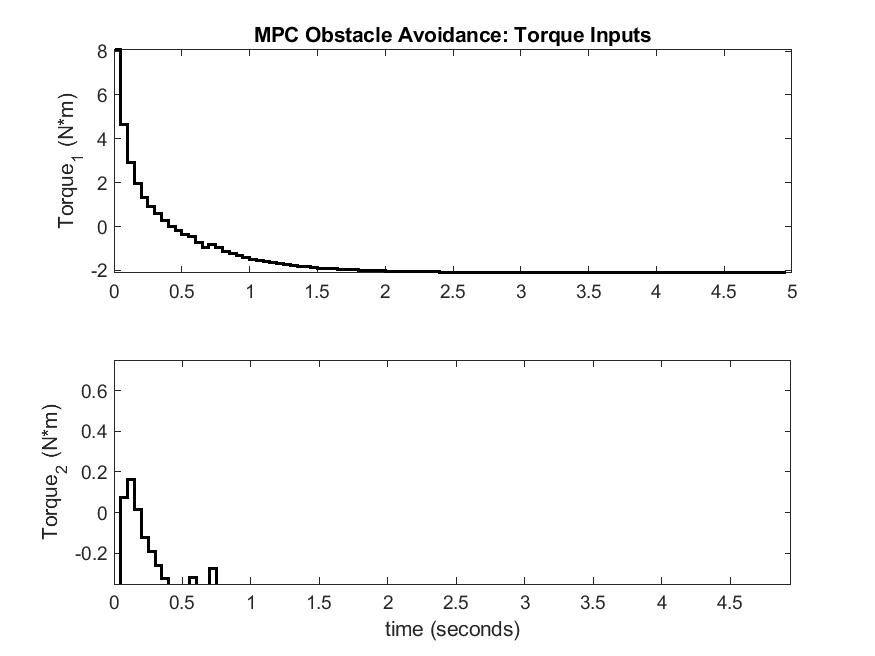
\includegraphics[width=.43\linewidth]{OBS_Avoid_TEST/T6/torque} }}%
    % \qquad
    % \subfloat[\centering label 4]{{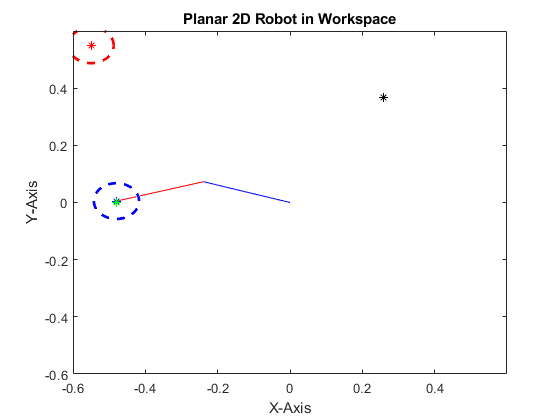
\includegraphics[width=.43\linewidth]{no_obj_path_final} }}%
    \caption{Obstacle Avoidance Control via MPC}%
    \label{fig:obs_avoid_control_action}%
\end{figure}


\begin{figure}[ht]%
    \centering
    \subfloat[\centering label 1]{{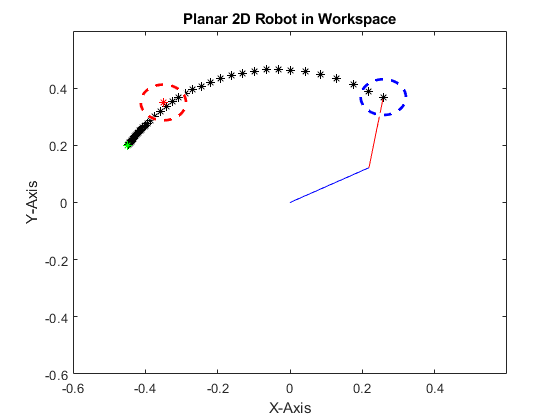
\includegraphics[width=.43\linewidth]{MPC_w_Obs_Avoid/path_1} }}%
    \qquad
    \subfloat[\centering label 2]{{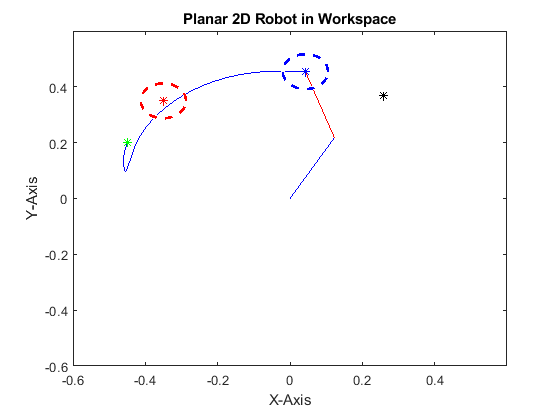
\includegraphics[width=.43\linewidth]{MPC_w_Obs_Avoid/path_2} }}%
    % \caption{2 Figures side by side}%
    \\
    \subfloat[\centering label 3]{{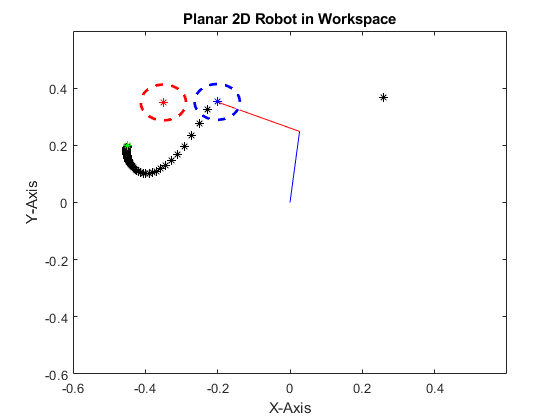
\includegraphics[width=.43\linewidth]{MPC_w_Obs_Avoid/path_3} }}%
    \qquad
    \subfloat[\centering label 4]{{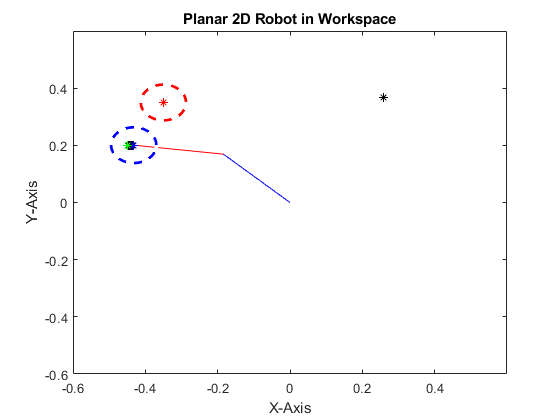
\includegraphics[width=.43\linewidth]{MPC_w_Obs_Avoid/path_final} }}%
    \caption{Obstacle Avoidance Control System}%
    \label{fig:obs_avoid_path}%
\end{figure}







\subsubsection{Infeasible Goal Pose (Constraint Violation)}

\begin{figure}%
    \centering
    \subfloat[\centering label 1]{{\includegraphics[width=.43\linewidth]{MPC_sys_Constraints_violation/T4_X_init_25_45_0_0_X_ref_260_n15_0_0/pos} }}%
    \qquad
    \subfloat[\centering label 2]{{\includegraphics[width=.43\linewidth]{MPC_sys_Constraints_violation/T4_X_init_25_45_0_0_X_ref_260_n15_0_0/vel} }}%
    % \caption{2 Figures side by side}%
    \\
    \subfloat[\centering label 3]{{\includegraphics[width=.43\linewidth]{MPC_sys_Constraints_violation/T4_X_init_25_45_0_0_X_ref_260_n15_0_0/tor} }}%
    % \qquad
    % \subfloat[\centering label 4]{{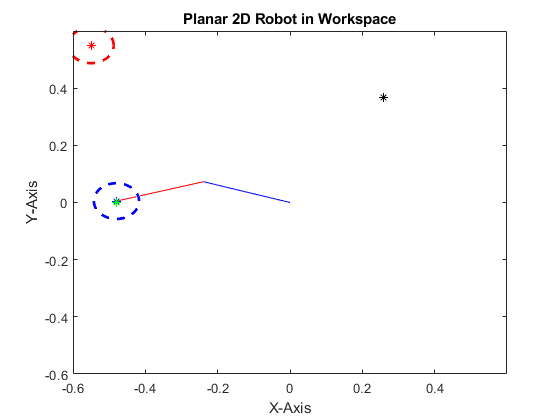
\includegraphics[width=.43\linewidth]{no_obj_path_final} }}%
    \caption{Infeasible Goal MPC}%
    \label{fig:infeasible_goal}%
\end{figure}

\subsection{Planner Results}

\subsubsection{Joint Paths}

\begin{figure}%
    \centering
    \subfloat[\centering label 1]{{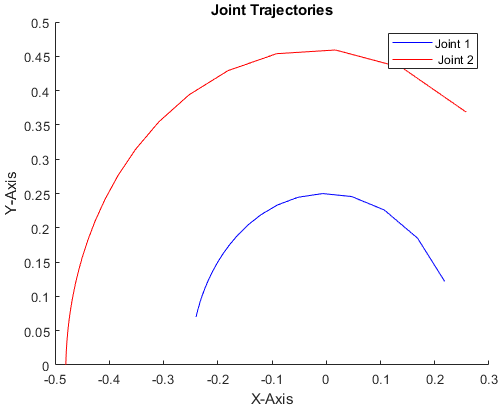
\includegraphics[width=.43\linewidth]{EndEffector_Path/p2p} }}%
    \qquad
    \subfloat[\centering label 2]{{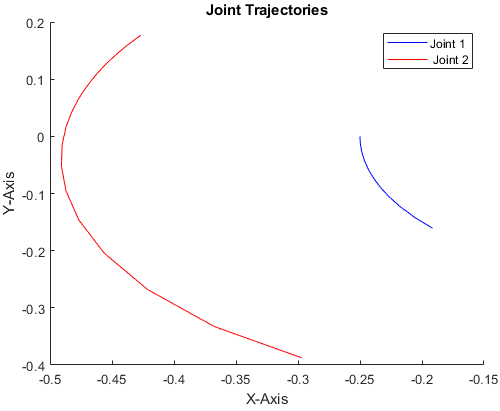
\includegraphics[width=.43\linewidth]{EndEffector_Path/p2p2} }}%
    \caption{Nominal System Joint Paths}%
    \label{fig:joint_path}%
\end{figure}

\subsubsection{End Effector Paths }

\section{Discussion}

\subsection{Control}

0 Fully controllable environment \\
1 MIMO formulation is intuitive \& easily extended to nonlinear systems (2D-3D)\\
2 Relatively responsive control authority\\
3 Respects system constraints (Actuator limits, range of motions)\\
4 Relatively simple to implement a crude form of obstacle avoidance (cost penalty or extra constriants.)\\
    4.1 Unreliable time till solution\\
    4.2 Highly sensitive to obstacle placement\\
    4.3 Poor tuning can lead to oscilatory behavior\\
    4.4 Can struggle to converge to final solution even if clear of obstacle (tuning?)\\
5

\subsection{Planning}

Possible To use MPC as a supervisory controller/planner for other\\

MPC planner is able to update the best path (given the current state) and can account for model uncertainties or object/obstacles in the direct path.\\

Planning with MPC allows the planner to track smoothly though the optimal state horizon which can then be leveraged by other controllers ...etc. which function at faster speeds than the base MPC controller could.\\

Unlike the most commonly used path planning algorithms (A*, Djikstra, RRT, RRT*, PRM, D*, and other discretized, graph, or heuristic search algorithms, such as Artifial potential fields) Path planning with MPC is a very control theoretic approach.\\

While the use case seen in this paper is not very impressive, predicting and controlling the path which the end effector of a robot takes from one position to another can quicker be seen in the three dimensional case where discretizing the entire feasible can be computationally intensive.\\





\section{Conclusion}
The conclusion goes here.


\section*{Acknowledgment}


The authors would like to thank Mountain Dew and his matress for constant support and comfort.



\ifCLASSOPTIONcaptionsoff
  \newpage
\fi

\cite{craig_introduction_2005}
\cite{khalil_nonlinear_2002}
\cite{rawlings_model_2017}
\cite{armstrong_explicit_1986}
\cite{ogata_modern_2010}
\cite{meriam_engineering_1993}
\cite{greenwood_advanced_2006}
\cite{borrelli_predictive_2017}
\cite{boyd_convex_2004}
\cite{slotine_applied_1991}

% \printbibliography

\begin{IEEEbiography}[{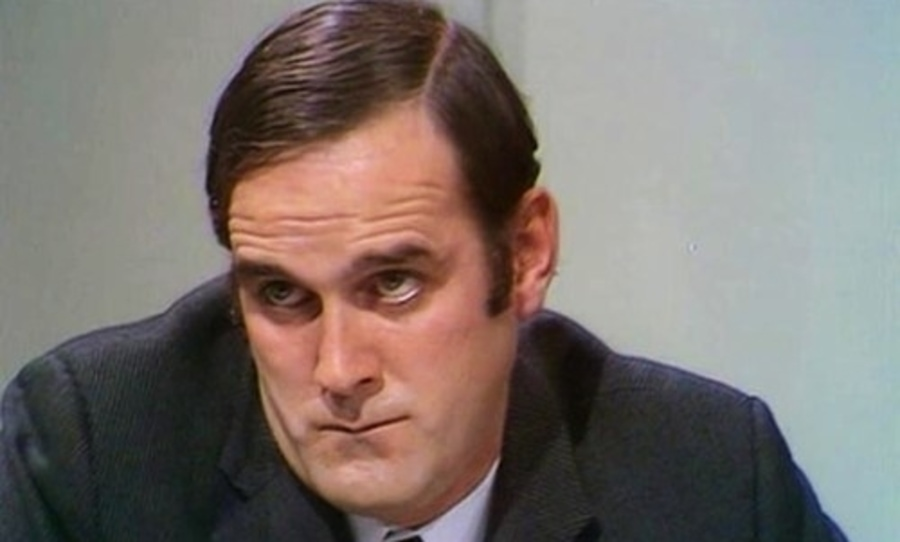
\includegraphics[width=1in,height=1.25in,clip,keepaspectratio]{monty1}}]{Jonathan Dorsey}
  I've already told you once. It is an ex parrot. Its has ceased to be. Recieved his Bachelors Degree in Mechanical Engineering from the San Jose State University. With a focus on mechatronics and control systems, he has developed an interest in reinforcement learning, computer vision, and control and design of autonomous systems.
\end{IEEEbiography}



\end{document}
